\section{Publish/Subscribe}
Many-to-many:
For communication,
For coordination,
$M$: data sources (publishing C) $n$: data sinks (subscribing C)
C \bluetext{decoupled} and do not know each other $\leftrightarrow$ tightly coupled Observer Design Pattern:
Removes explicit dependencies, 
Reduces coordination synchronization, 
Increases scalability of dis. SY,
Creates highly dynamic(frequent add/remove) decentralized SY,
Decoupling in three dimensions(\bluetext{Space Dec.}
No need for C (publishers \& subscribers) to hold references or know each other, C physically distributed,
\bluetext{Time Dec.}C not to be available same time(Event in Buffer)
\bluetext{Synchronization Dec.}Control flow not blocked by the interaction)
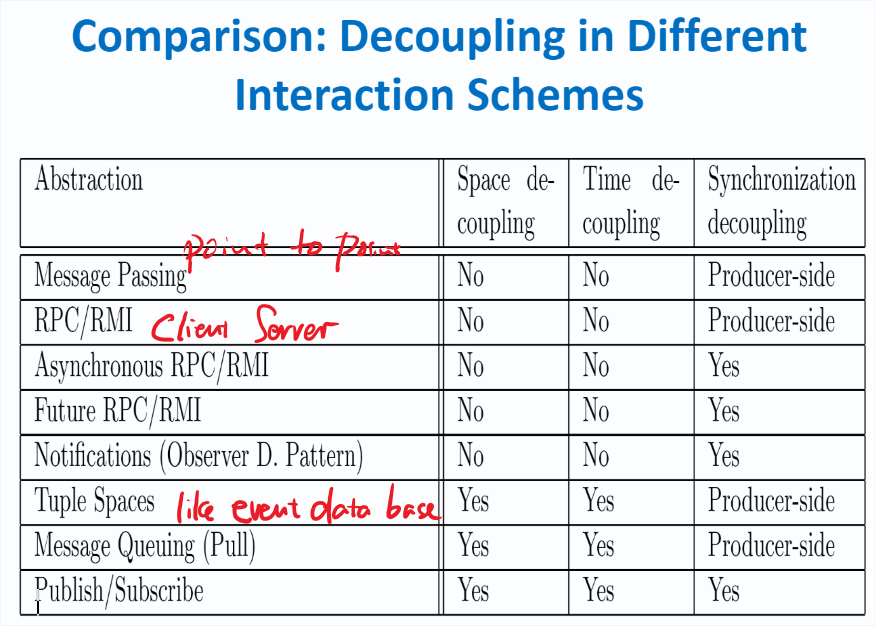
\includegraphics[width=\linewidth]{chap9_1.png}
\btext{Pub/Sub Models}: Content-based, Channel-based(non-hierarchical), Topic-based(hierarchical, sport new USA)
\btext{Matching\&Filtering in Content-based}:
event(Publication) $e$, set of subscriptions $S$, find all subscription $s\in S$ matching $e$.
\bluetext{Subscription}: Boolean function over predicates
\bluetext{Publication(event)}: Sets of attribute-value pairs
\btext{Two-phased Matching Algo.}
1.Match all predicates (\bluetext{Predicate Matching Phase})
2.Match subscriptions from results of Phase 1 (\bluetext{Subscriptions Matching Phase})
\btext{1.Predicate Mat.P.}:  set $P$ of predicates and event $e$, 
identify all satisfied predicates $p$ of $P$ $\rightarrow$ Predicate bit vector,
Hash key = attribute name
\bluetext{General Purpose Data Structure}: for single attribute: 4 ordered linked list(b tree) for $=, <, >, !=$ operators, $O(n)$ all events \& lists
\bluetext{Finite Predicate Value Domain Types}: huge matrix eg $1000 * 4\;for Price \in [1, 1000]$,
1000 for price, 4 for operators, entry lookup $m[i][j]=O(1)$
\btext{2.Subscription Mat.P.: Counting Algo}
\textbar
\btext{Content-based Routing}
1.Advertisements (schema or types,data sources) \redtext{Boradcast},
2.Publications \& events (data sources))
\begin{CJK*}{UTF8}{gbsn}
\redtext{根据上一步Broker's Subscription走}
\end{CJK*},
3.Subscriptions (query, data sinks)
